\chapter{Application architecture}
\label{sec:application-architecture}
	
%	TODO: rewrite intro
    This chapter covers the application architecture. We present here the essential services and application components that enact the current and the new life-cycle processes.

	\section{Prototypical application structure}
	
	This section presents the application architecture from the solution architecture point of view. A generic solution architecture is depicted in Figure \ref{fig:application-view}.
	
	The application architecture presented covers the application as a ``white box'', its internal component structure, services and interfaces with adjacent applications. Typically the solutions architecture takes the technology aspects into account, accounting for parts of the infrastructure.
	
    \begin{figure}[h]
		\centering
		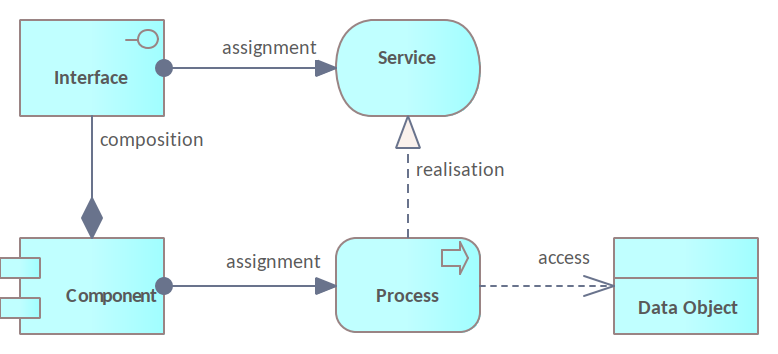
\includegraphics[width=.6\textwidth]{images/views/Application view.png}
		\caption{The prototypical application structure view}
		\label{fig:application-view}
	\end{figure}

	The central element of the application architecture is the \textit{application service}, which represents application behaviour or functionality. The application services, from an inter-layer perspective, serve the processes in the business layer and provide support for their realisation. 
	
	The application services are realised through application processes. The processes have application components assigned to them signifying their place of encapsulation. Application components are modular and replaceable blocks encapsulating implementation of application services and functionalities. In practice, for clarity, we take a shortcut, and say that the application services are realised through \textit{application components} directly.
	
	Components are said to expose interaction \textit{interfaces} which are modelled, in ArchiMate, as proper parts of the components. The interfaces are assigned to services signifying how the latter are to be accessed and consumed. 
	
	Also, components, as well as processes they encapsulate, access \textit{data objects}, which are passive components of the application architecture.

	The solution architecture presented in this section is an adaptation of the generic architecture. Here we focus on presenting what application services are used to support each business process. Moreover, we are interested in grasping the difference in the application layer, between the current and new versions of the business processes. 
	
	To do so, we split the application view diagrams into three vertical lanes. The left lane hosts the current version of the business process as well as the application services and components that are used to support it. In the right lane, we place the new business process and the new application services and components that will have to be adopted for the digital transformation. The middle lane hosts the services and components that are are currently employed and will be carried over into the new application architecture: they are common to both the current and new architectures.

	Below we present an overview of the application architecture, in terms of services alone, depicting how the asset life-cycle stages are served.	
	
	\section{LAM specific application architecture}

	This section presents the application architecture for services developed in the context of LAM\#2 project. In Section \ref{sec:application-lifecycle} these applications will be placed into the context of asset lifecycle process described in Section \ref{sec:asset-lifecycle}. 
	
	The project specific tools are \textit{the transformation tool}, \textit{the validation tool} and \textit{the online (dissemination) tool}.
	
	\subsection{LAM transformation tool}
	\label{sec:transformation-tool}
		
	First of the three tools, is the transformation tool from structured RDF data into human readable representations. This tool contributes directly to the goal of producing and dissemination the LAM data for end-user consumption on the OP Portal. This tool is used during the release phase of the lifecycle as will be explained in Section \ref{sec:release}.	
	
	Figure \ref{fig:app-transformation-tool} depicts the application architecture, with LAM transformer component in the centre of the diagram.
	
	
    \begin{figure}[!h]
		\centering
		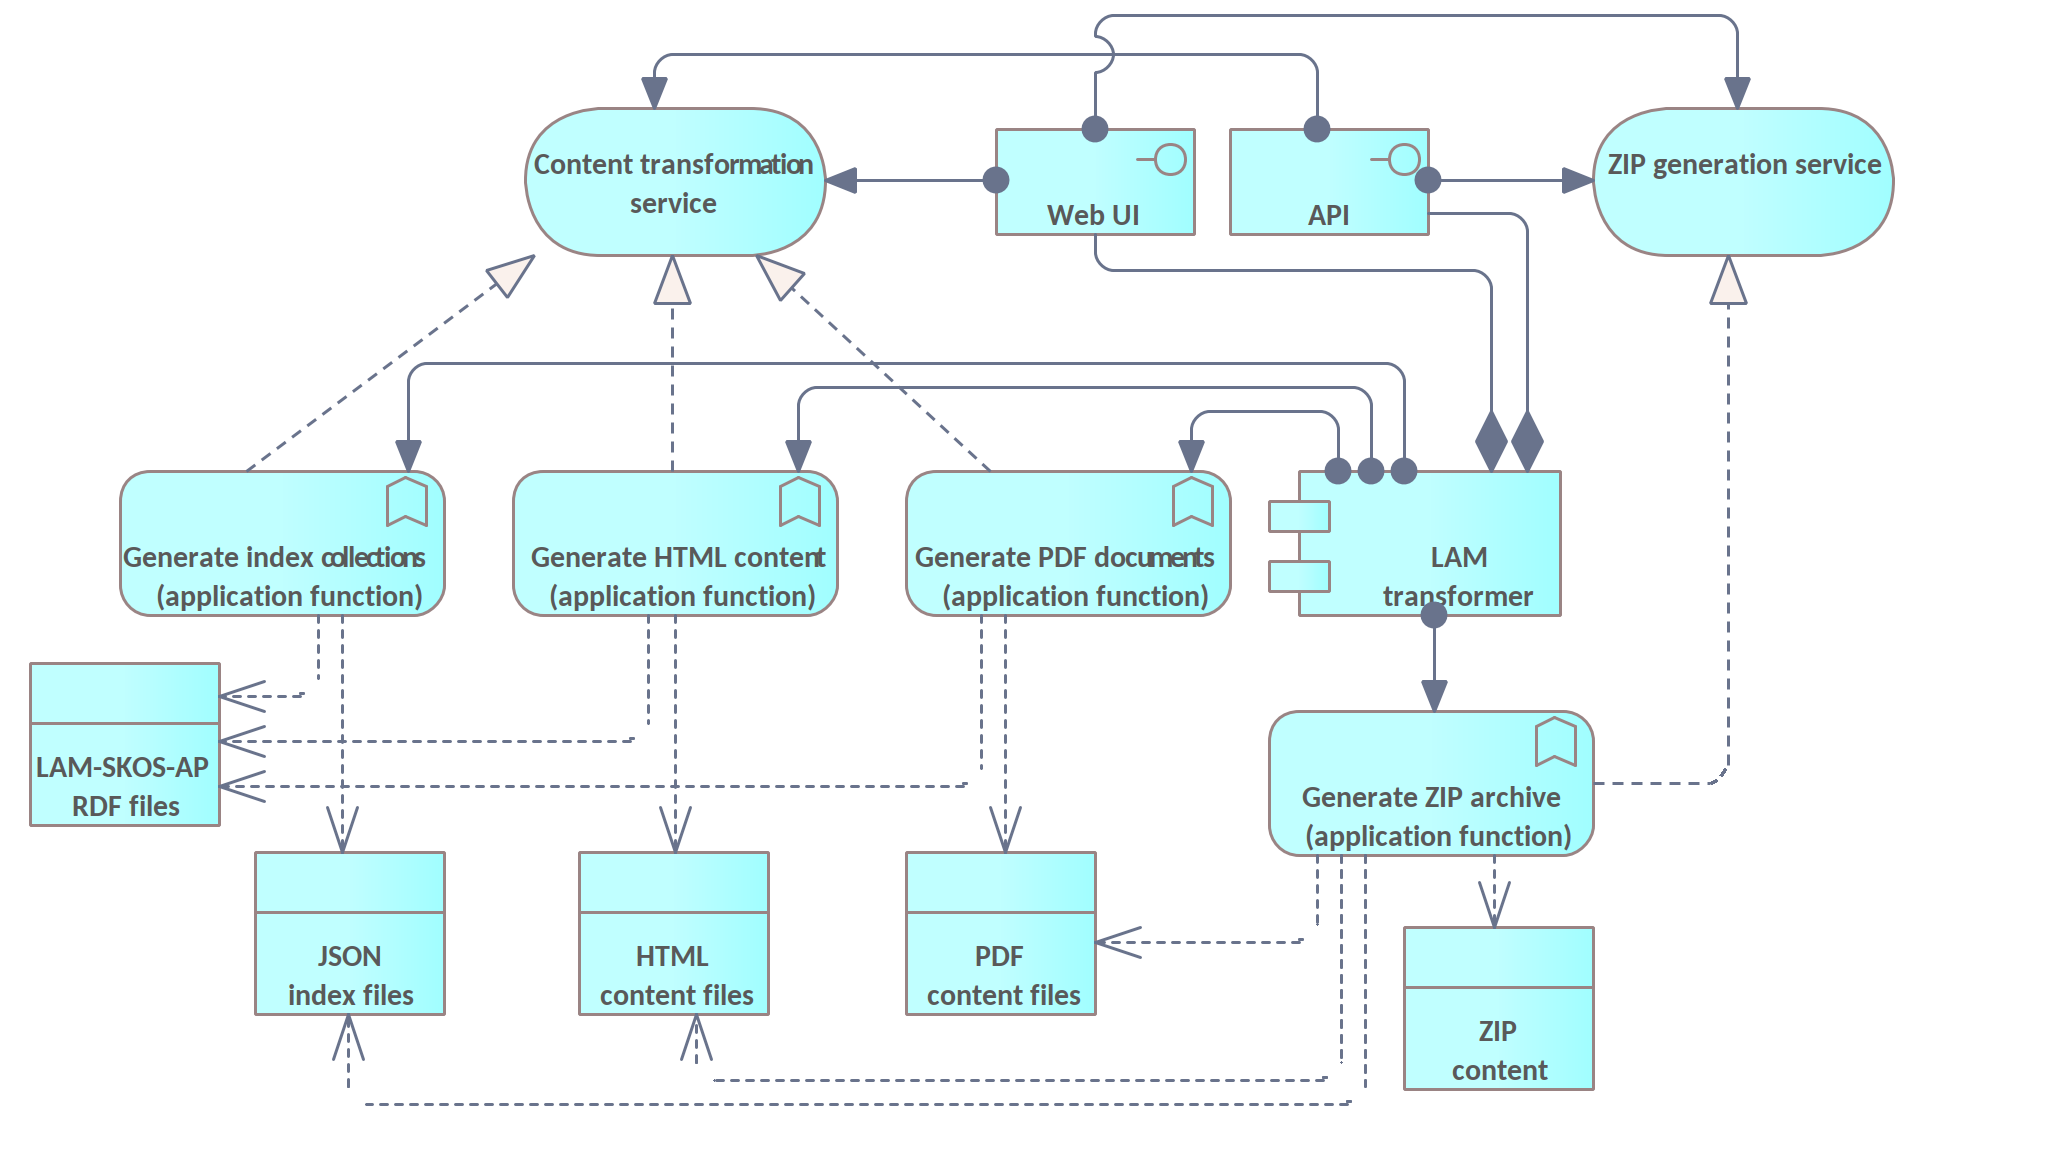
\includegraphics[width=.98\textwidth]{images/application/Content transformer.png}
		\caption{LAM transformation tool application architecture}
		\label{fig:app-transformation-tool}
	\end{figure}



	The main service this application exposes is the content transformation, positioned on the top of the diagram. This service is exposed through two interfaces: a web graphical user interface and an application programming interface. This service is realised by three application functionalities: generation of the HTML representation, generation of the PDF representation and generation of JSON indexes. The first two representations are meant to be distributed as such for the end-user consumption, while the indexes are meant to enable the search functionality provided by the OP Portal. The input taken by these functionalities shall be structured according to LAM-SKOS-AP\cite{lam-skos-ap-2019}.
	
	In order to facilitate the transmission of the artefacts generated by the LAM transformer, an additional service is foreseen, which aggregates the results of the transformation service into a ZIP archive. In the next section is described the LAM online tool, which ingests the ZIP archive and disseminates its content on a web interface. 
	
	\subsection{LAM online tool}
	
	The LAM online tool is a mini-website hosted within the OP Portal ecosystem. Its main services are the content import, content consultation and content search. Figure \ref{fig:app-online-tool-ingestion} depicts the architecture supporting the content ingestion. 
	This tool is used during the publication and consumption phase of the lifecycle as will be explained in Section \ref{sec:publication}.
		
    \begin{figure}[!h]
		\centering
		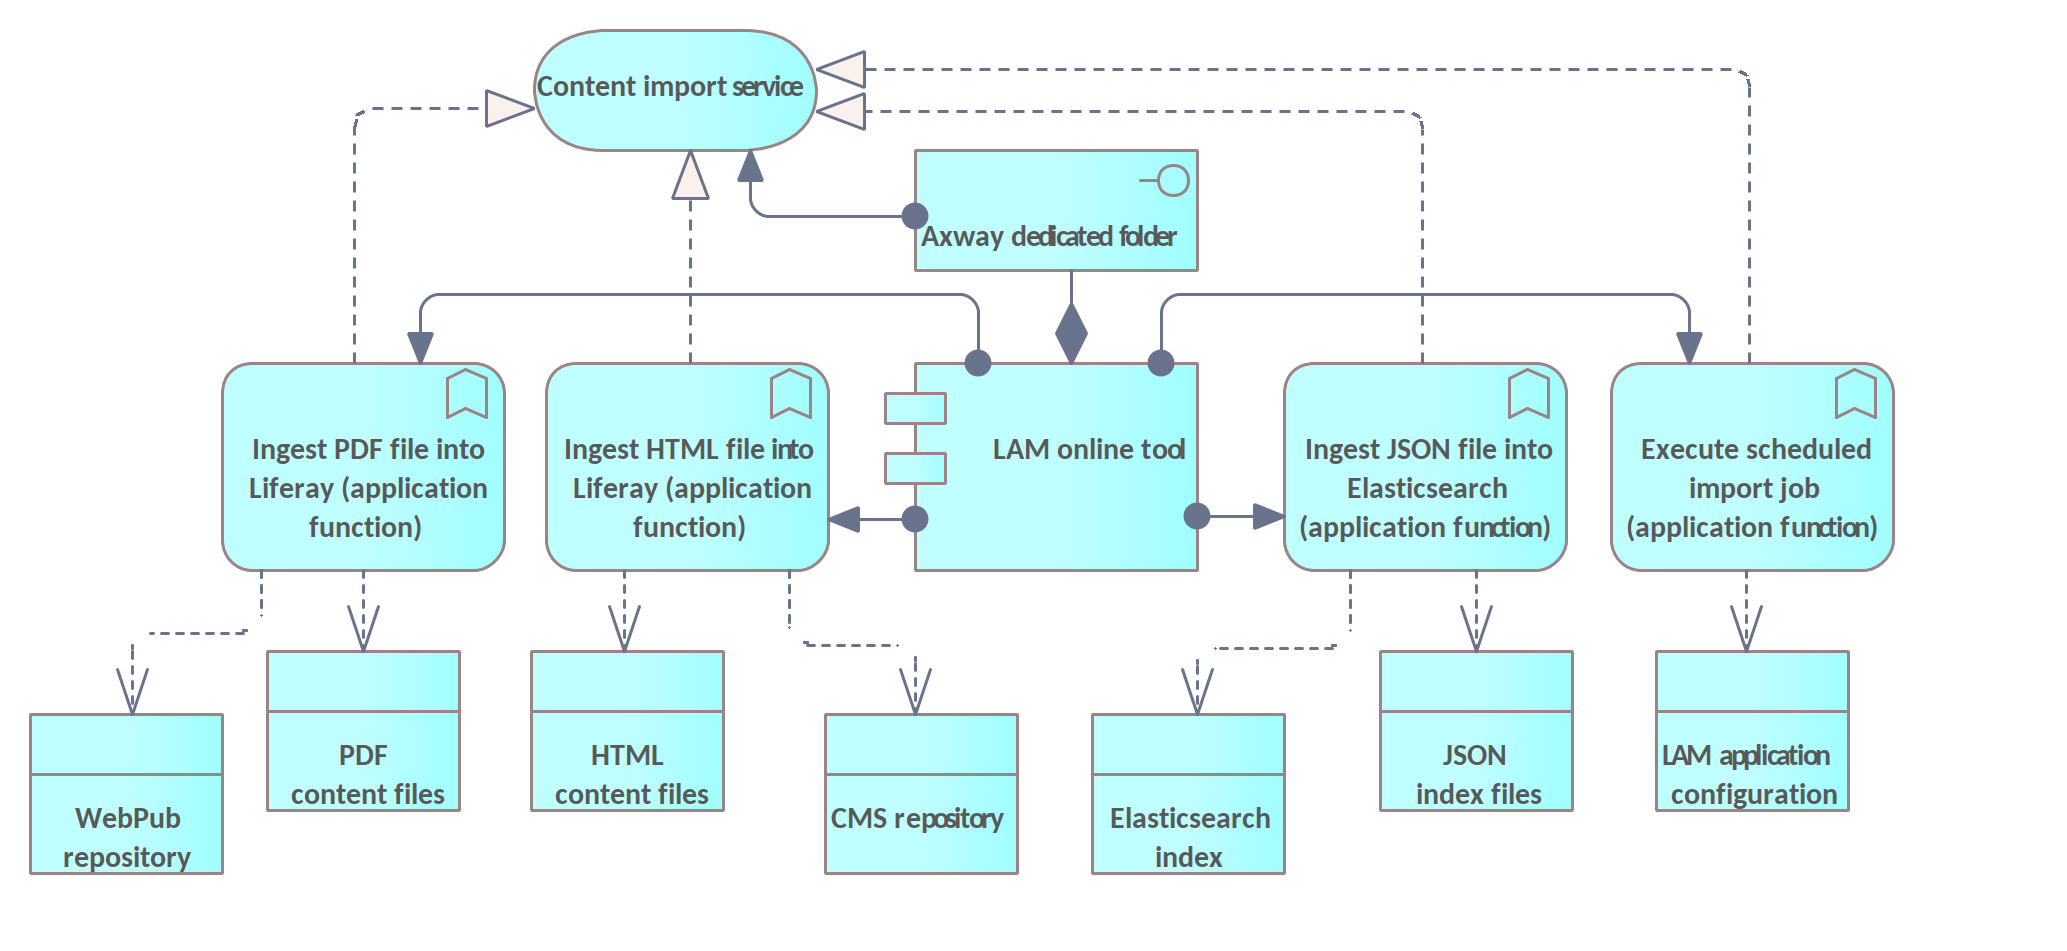
\includegraphics[width=.98\textwidth]{images/application/Online tool - import.png}
		\caption{LAM online tool application architecture: content import service}
		\label{fig:app-online-tool-ingestion}
	\end{figure}	

	The import service is exposed through a dedicated Axway folder where a scheduled job regularly checks for new content. As soon as new content is placed there the ingestion functionality starts. The expected input is the ZIP archive containing the PDF, HTML and JSON content. When this archive is unpacked each of these representations is treated accordingly for different purposes.
	
	The content import service is realised through four application functions assigned to the LAM online tool component (see central area in Figure \ref{fig:app-online-tool-ingestion}). The PDF files are ingested into a WebPub repository using Liferay framework. The HTML files are ingested into a Liferay CMS repository. The JSON index files are loaded into the Elasticsearch index. The import operation is triggered by running a scheduled task. 
	
	
	The LAM online tool is conceived as a mini-website in the OP Portal. The main dissemination method is a Web user interface, exposing two services: the content consultations ervice and the content search service. 
	
    \begin{figure}[!h]
	\centering
	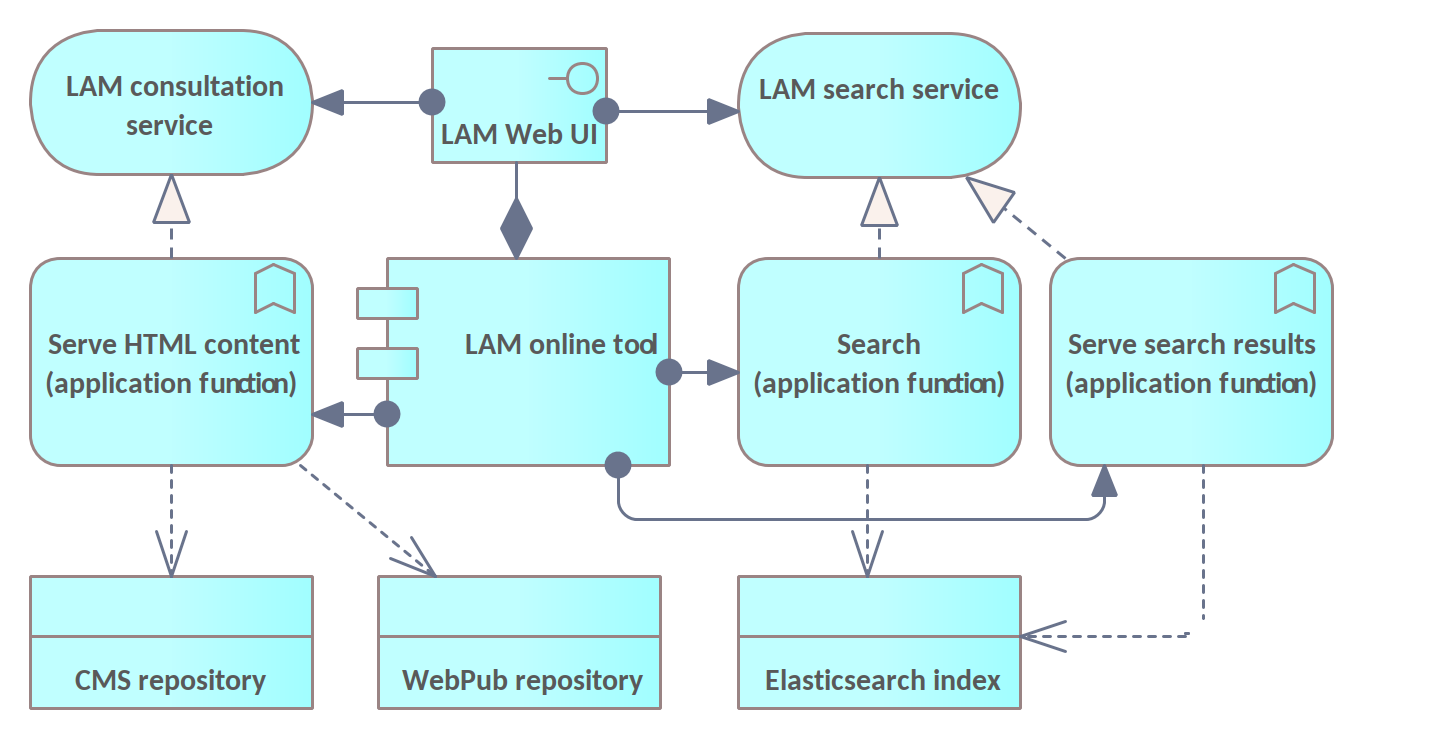
\includegraphics[width=.78\textwidth]{images/application/Online tool - dissemination.png}
	\caption{LAM online tool application architecture: content dissemination services}
	\label{fig:app-online-tool-dissemination}
	\end{figure}
		

    \begin{figure}[!h]
	\centering
	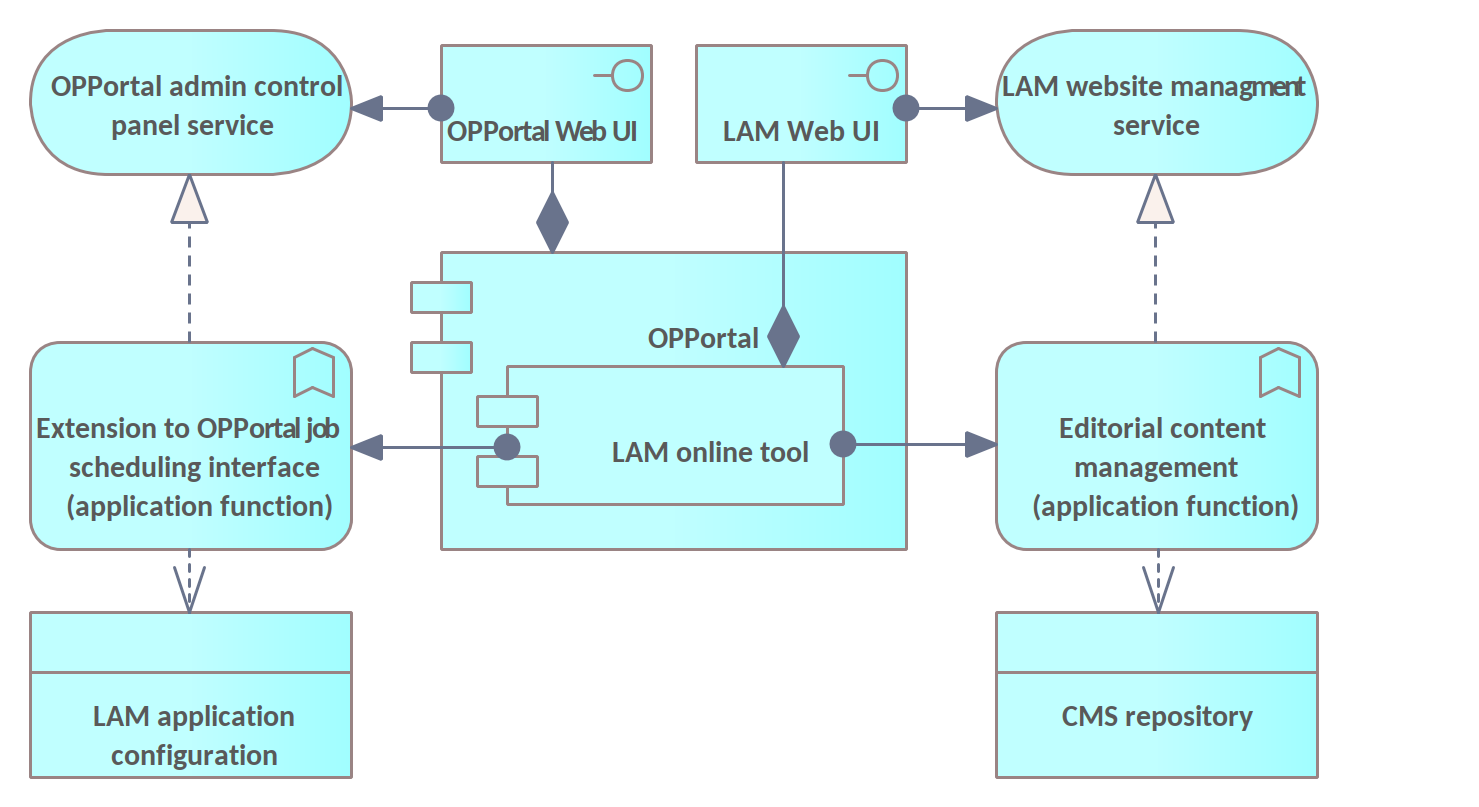
\includegraphics[width=.67\textwidth]{images/application/Online tool - management.png}
	\caption{LAM online tool application architecture: administration services}
	\label{fig:app-online-tool-management}
	\end{figure}

	The search service is realised by Elasticsearch search functionality and serving the search results from the index and rendering them in a web interface. 
	
	The consultation service is realised by serving web pages from Liferay CMS and the PDF documents from WebPub repository. In addition there is a set of Liferay editorial pages exposing custom content, such as news, publication change notes, links to relates resources etc. These pages are edited through LAM website management console offered by Liferay framework. This service is depicted in Figure \ref{fig:app-online-tool-management}. 
	
	Another configuration that is available in the administration console is that of the scheduling task. This functionality constitute in fact an extension to the scheduling functionality available in the OP Portal. For this reason the configuration is exposed through OP Portal web interface. 
	
	\subsection{LAM validation tool}
	
	In Section \ref{sec:lam-maintenance-publication} was presented that structured LAM data are maintained using VocBench3 system. This system is versatile and well suited for the task, yet structural deviations from the designed model, LAM-SKOS-AP, are likely to happen. 
	The motivation for using the LAM validation tool is that after the data are exported from VocBench3 and fed as input to the LAM transformation tool, it is imperative that the data are valid. Otherwise, the LAM transformation tool may render unexpected results or behave in an unpredictable manner. 
	
 	\begin{figure}[!h]
		\centering
		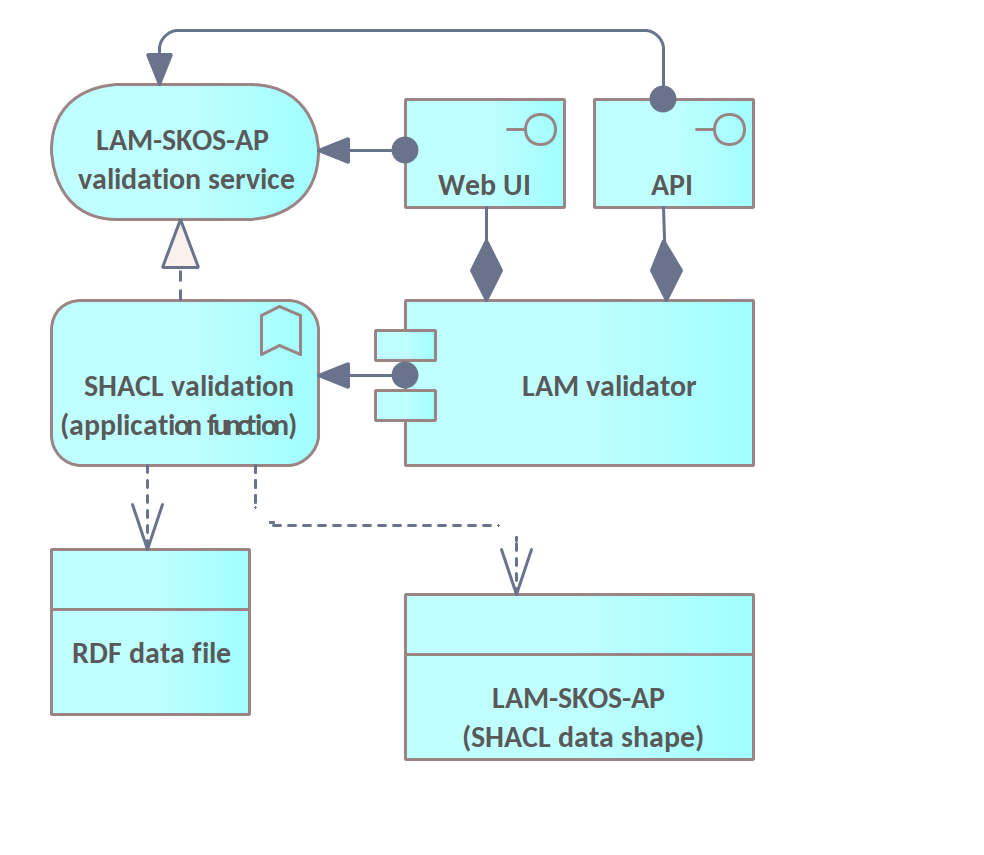
\includegraphics[width=.517\textwidth]{images/application/LAM Validator.png}
		\caption{LAM validation tool application architecture}
		\label{fig:app-lam-validator}
	\end{figure}

	In order to ensure that the transformation tool generates satisfiable results, the input data needs to be validated. This is a procedure preformed in the implementation phase, as will be shown in Section \ref{sec:implementation}. 
	
	Figure \ref{fig:app-lam-validator} depicts the LAM validator application architecture. It exposes a single service through a Web user interface and an API. The service is realised through a SHACL \citep{shacl-spec} validation functionality with a predetermined set of SHACL shapes - the LAM-SKOS-AP\citep{lam-skos-ap-2019} SHACL representation. Any RDF fine that is provided to the service is tested against this preset data shape. 

	\section{LAM lifecycle application architecture}
	\label{sec:application-lifecycle}
	
	In this section the lifecycle process describe din Section \ref{sec:asset-lifecycle} is connected to the application services and components realising them. Many of these services are available for usage, and describing them in detail is out of scope here. What is relevant to show here how the lifecycle processes are served and where the LAM specific applications are involved.
	
	\subsection{Evolution management}
	
	In the first stage of the asset lifecycle, the application requirements are limited to client
communication and the request documentation services as depicted in Figure \ref{fig:app-evolution-management}. The email service is realised by the Outlook software. Issue management is realised by the Jira system.
	
    \begin{figure}[!h]
		\centering
		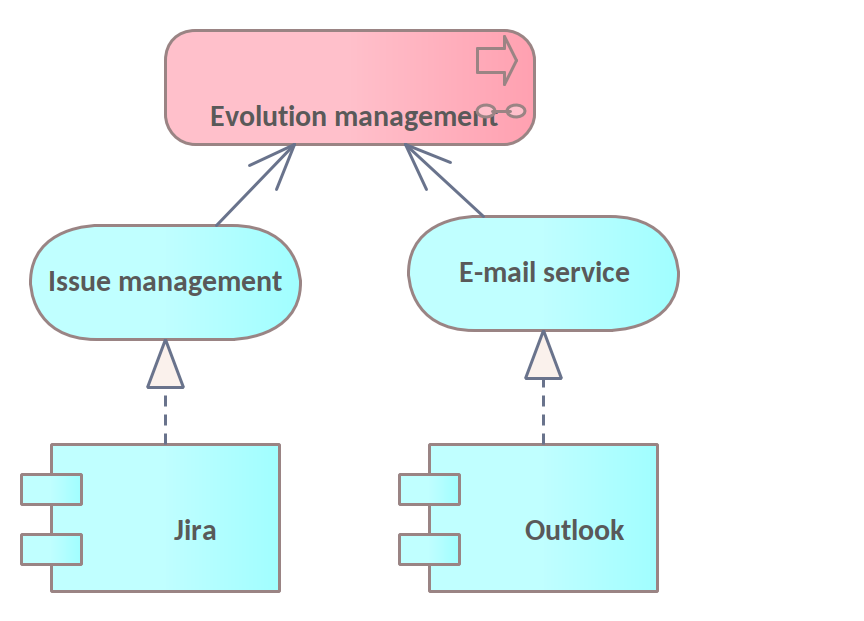
\includegraphics[width=.45\textwidth]{images/application/lifecycle/Evolution.png}
		\caption{Application services and component that serve evolution management lifecycle stage}
		\label{fig:app-evolution-management}
	\end{figure}

	
	\subsection{Implementation}
	\label{sec:implementation}
	
	The implementation stage is the first place where considerable number of application services are involved. This is depicted in Figure \ref{fig:app-implementation}. 
	
    \begin{figure}[!h]
		\centering
		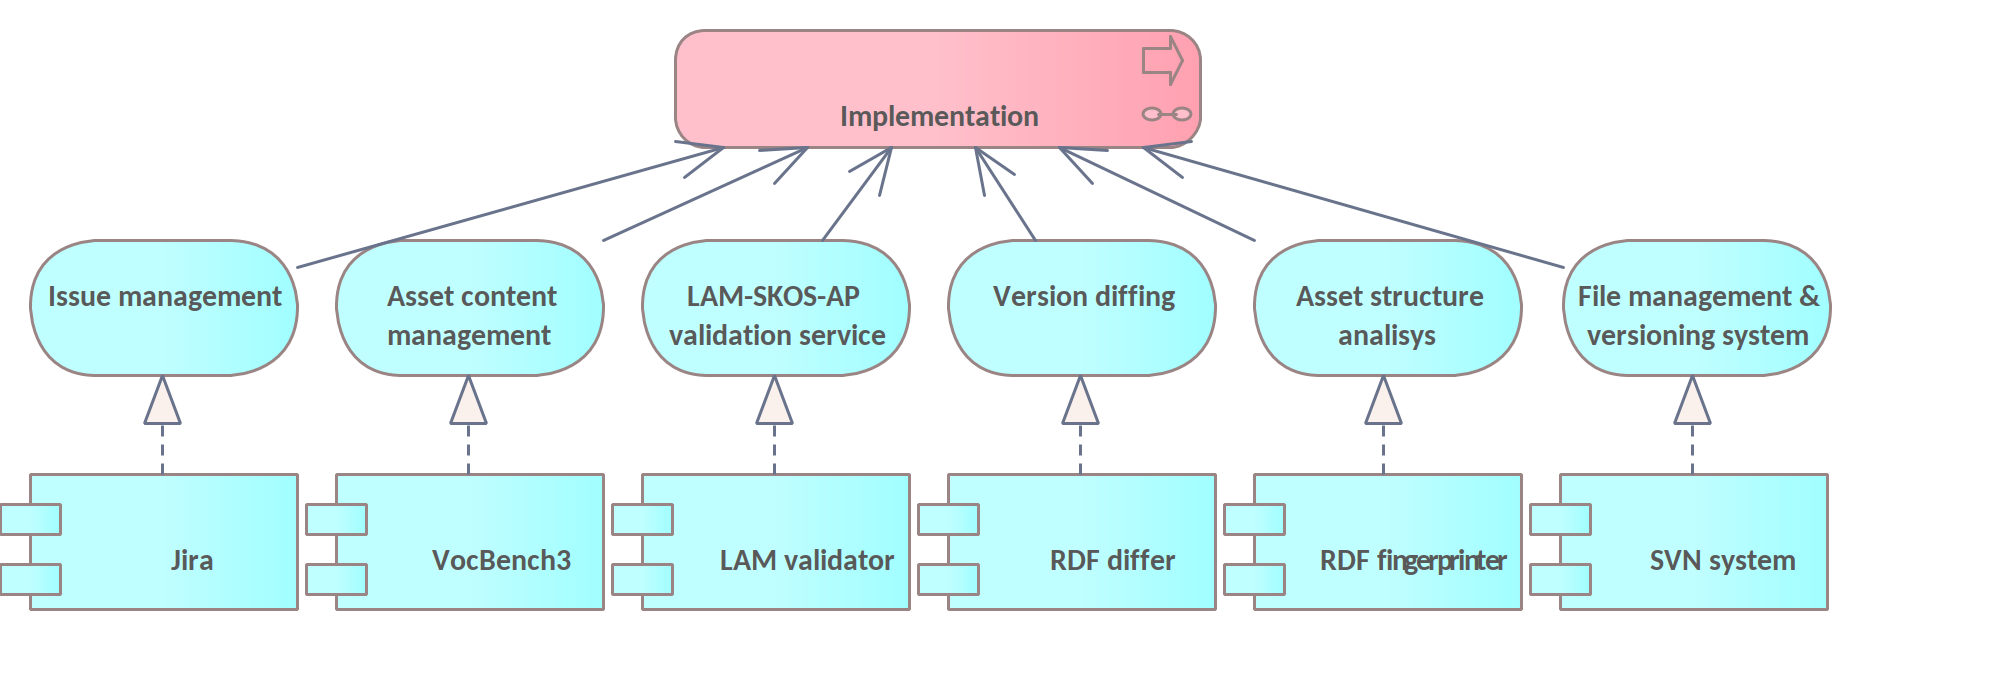
\includegraphics[width=.95\textwidth]{images/application/lifecycle/Implementation.png}
		\caption{Application services and component that serve implementation lifecycle stage}
		\label{fig:app-implementation}
	\end{figure}
	
	The issue management, just like in the case of evolution management stage, is realised by Jira system. The content editing is realised through VocBench3 system, and once the editing operation of complete, the content is exported for further processing. First it is validated using the LAM validation tool. Then it is compared to a previous version to check whether the set of changed done corresponds to what is requested in the Jira ticket. The asset is also fingerprinted, to asses for possible structural deviations, not covered by the validation service. It is important to mention that the LAM asset is stored using a file management and versioning service realised by the SVN system. This file based repository is used as a medium to transit the assets through all the lifecycle phases, except consumption. 

	\subsection{Validation}
	
	The stages following the implementation is validation. The services involved in this phase are issue management and file management service depicted in Figure \ref{fig:app-validation}.
		
	 \begin{figure}[!h]
		\centering
		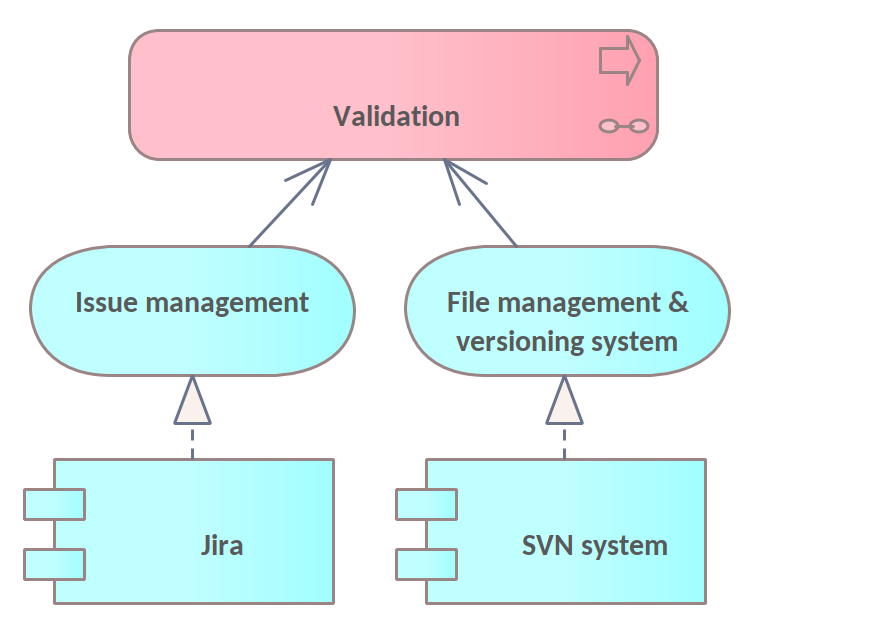
\includegraphics[width=.5\textwidth]{images/application/lifecycle/Validation.png}
		\caption{Application services and component that serve validation lifecycle stage}
		\label{fig:app-validation}
	\end{figure}	
	
	Generation fo validation artefacts is done during the implementation stage and stored in SVN. This stage is designed to allow a second person to check whether the implementation is done correctly following the ``four eye principle''. The validation office simply needs to access the validation artefacts from SVN and compare to the original change request. 
	
	\subsection{Release}
	\label{sec:release}
	
	Once the asset has been validated it is considered fit for publication. To do so it has to be transformed into all formats and representations necessary for the dissemination platforms and for final consumption by the end-users. 
	
	 \begin{figure}[!h]
		\centering
		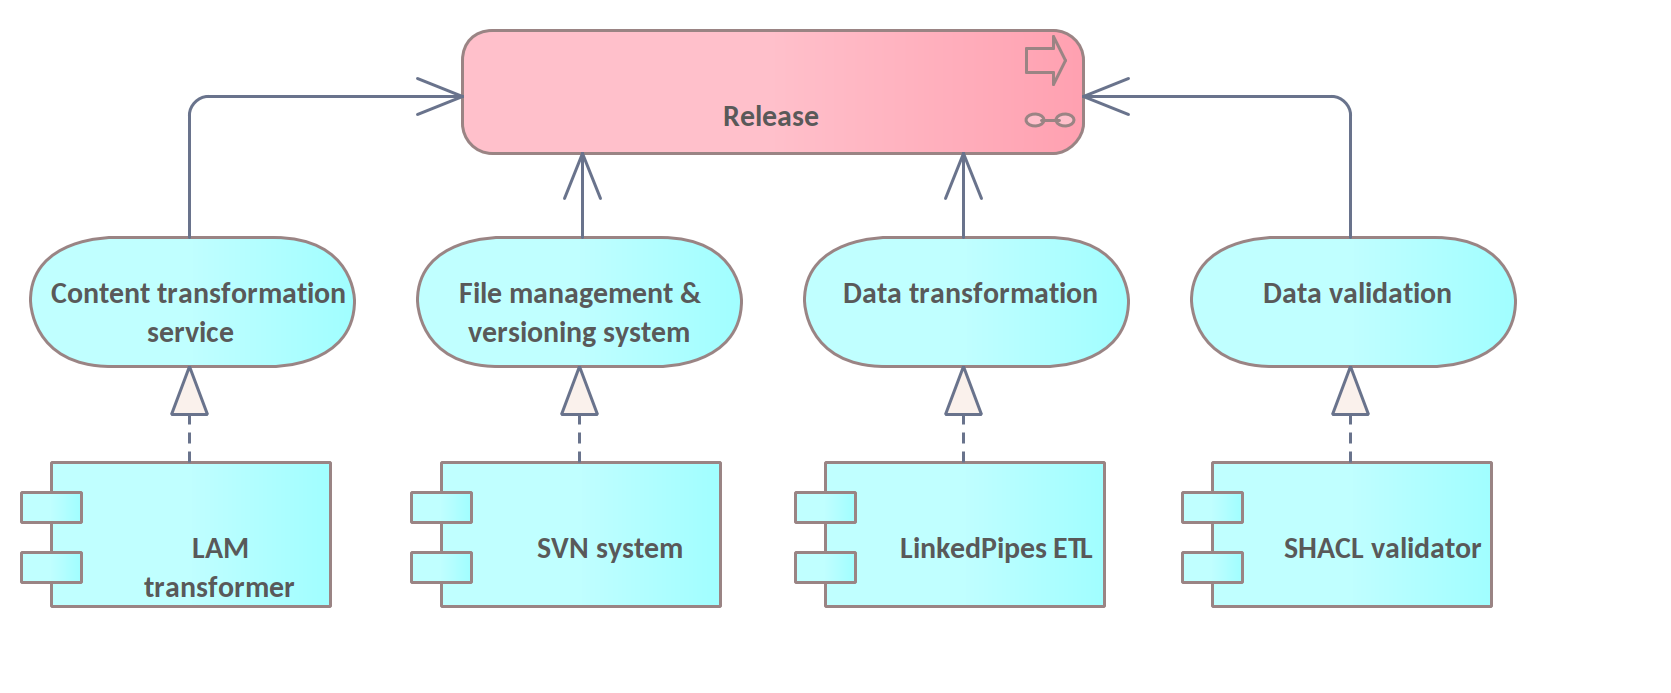
\includegraphics[width=.8\textwidth]{images/application/lifecycle/Release.png}
		\caption{Application services and component that serve release lifecycle stage}
		\label{fig:app-release}
	\end{figure}

	In this stage, depicted in Figure \ref{fig:app-release}, general data transformation service is involved, but also LAM transformation tool that was described in Section \ref{sec:transformation-tool}. The input and output of the transformations are red from and written back into the SVN system. Optionally a data validation service is used to perform a technical assessment before being sent to the dissemination systems.
	
	\subsection{Publication}
	\label{sec:publication}
	
	The publication stage is the last one in the asset life-cycle process. Its application
architecture is depicted in Figure \ref{fig:app-transformation-tool}.
	In this phase, the assets are packaged and transmitted to the dissemination system. 
	
	 \begin{figure}[!h]
		\centering
		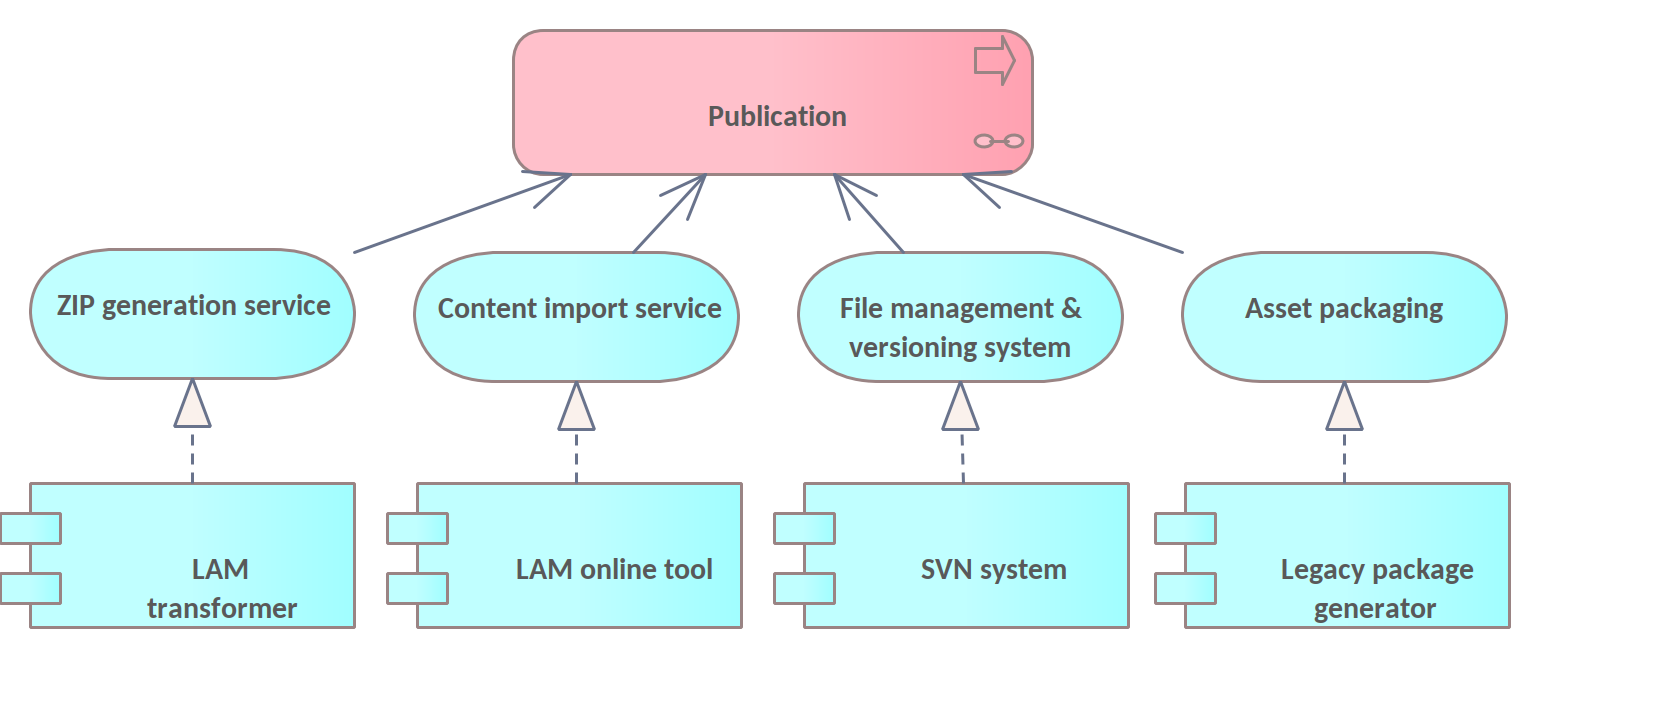
\includegraphics[width=.8\textwidth]{images/application/lifecycle/Publication.png}
		\caption{Application services and component that serve publication lifecycle stage}
		\label{fig:app-publication}
	\end{figure}

	The packaging is realised through two services. The ZIP generation service, realised by the LAM transformation tool, prepares the asset to be transmitted to the OP Portal system, where the LAM online tool is deployed. 
	
	The METS\citep{mets} asset packaging service it is realised by the legacy
	package generator which assembles in various ways asset artefacts as necessary for
partner dissemination systems and final consumers. This packaging specific to the Cellar system where the LAM data are published in machine readable format. 
	
	This brings us to the end of the application architecture description.